\chapter{Model architecture}
For our end-to-end SVG generation method, we build upon the work of~\citeauthor{ha2017neural} and use a similar bidirectional sequence-to-sequence variational autoencoder model~\cite{ha2017neural}.
We maintain a similar encoder and latent space architecture, but we modify the decoder to output parameters to four probability distributions instead of two: three Gaussian Mixture Models (GMMs) represent the three coordinates in the feature vectors, and one categorical distribution is used for modeling the pen state.
An overview of the model architecture is depicted in Figure~\ref{fig:architecture}.

\section{VAE modules}
Dual RNNs are used in the encoder module, one for forward and one for backward sequences of feature vectors, with each feature vector representing a single SVG command.
Both RNNs use LSTM cells with layer normalization, as introduced in~\cite{ba2016layer}.
After transforming an input SVG into a sequence of feature vectors $S = (S_1, S_2, \cdots, S_n)$, each $S_i$ is passed in to the encoder RNNs in the appropriate order.
The final hidden states of both RNNs, $h_\leftarrow$ from the backward encoder and $h_\to$ from the forward encoder, are concatenated to form a combined output $h$.
Assuming the latent space vector has dimension $n_z$, this output is then transformed into $\mu$ and $\sigma$ vectors using a fully connected layer (and an exponentiation operation to produce a non-negative $\sigma$) such that both vectors have dimension $n_z$.

\begin{figure}[h]
\centering
\caption[An overview of the basic SVG model architecture]{An overview of the basic SVG model architecture.
Although similar overall to~\cite{ha2017neural}, the model is adapted such that $y_i$ parameterizes three pen location GMMs and a pen state distribution.\label{fig:architecture}}
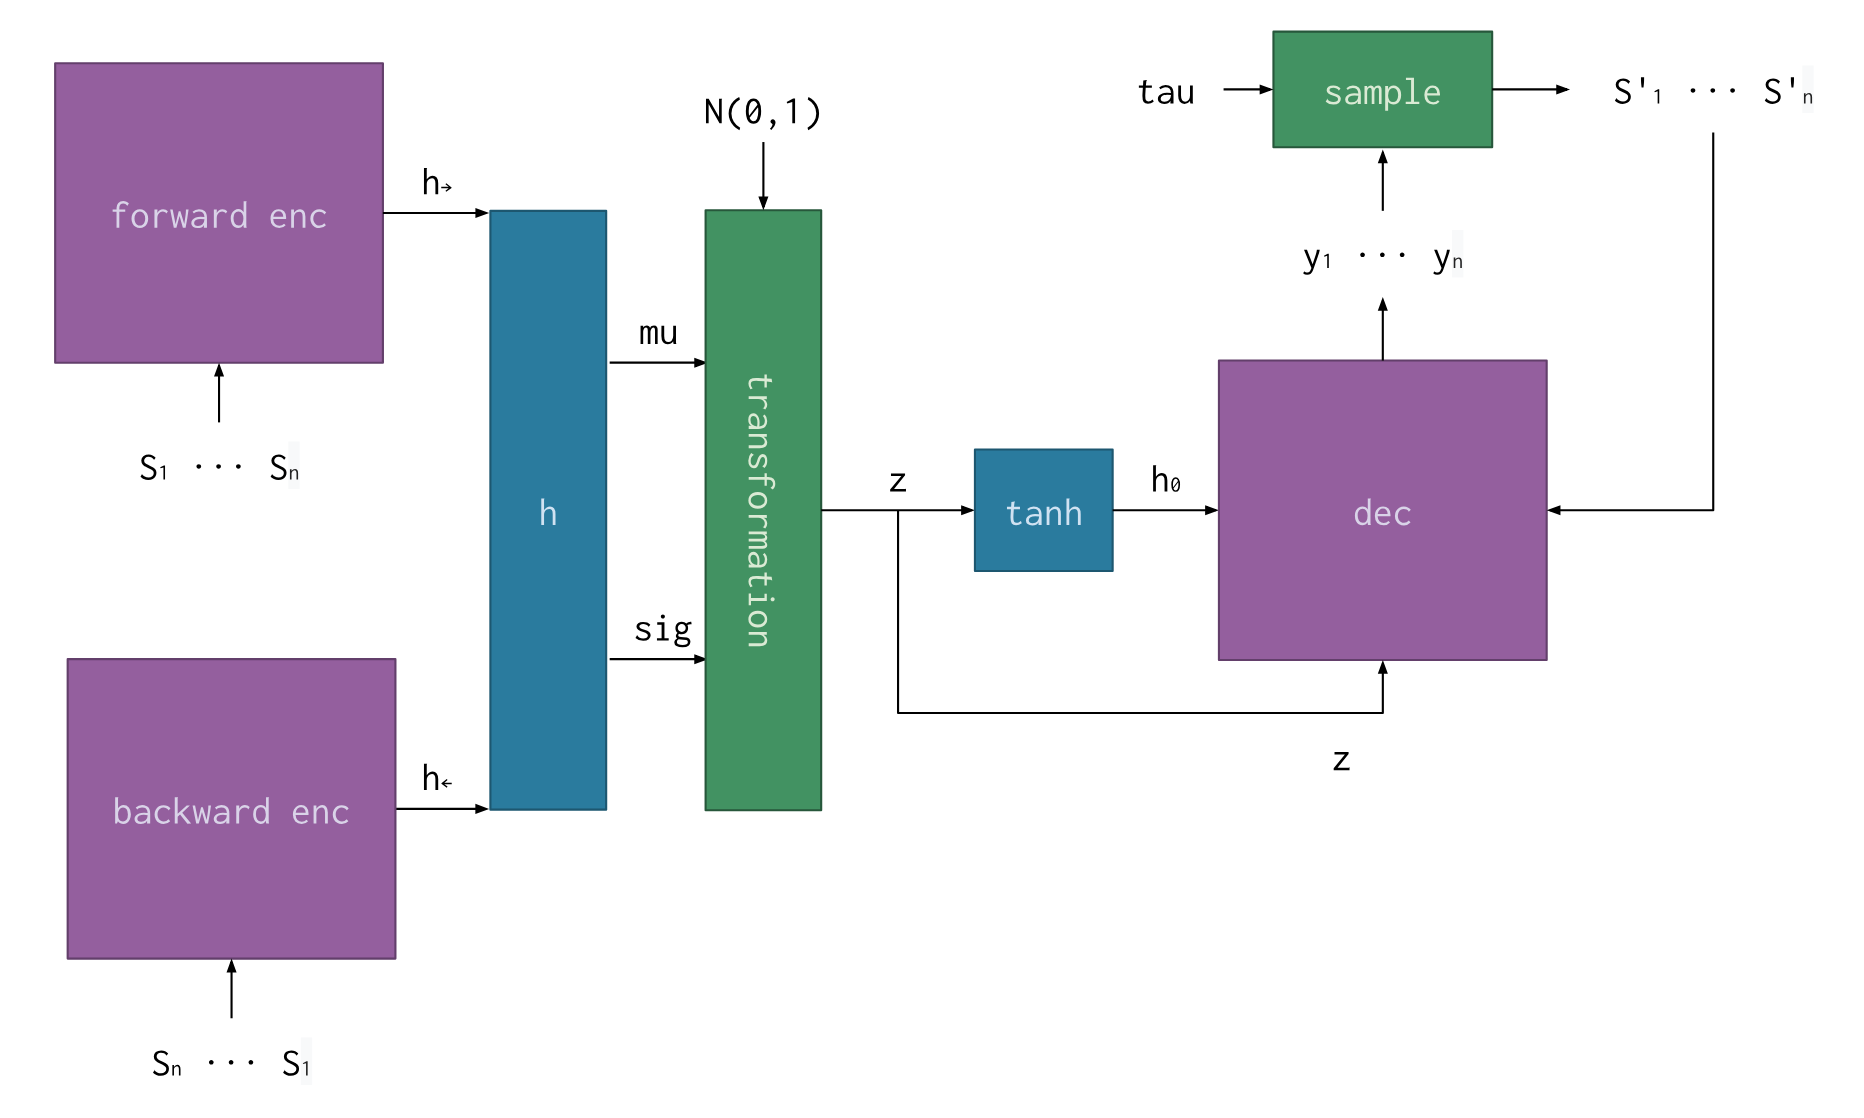
\includegraphics[width=\textwidth]{figures/architecture}
\end{figure}

The resulting $\mu$ and $\sigma$ vectors are combined with a vector $\mathcal{N}$ of $n_z$ normally distributed Gaussian samples from $\mathcal{N}(0,1)$ to create a random latent vector $z$, with $z = \mu + \sigma \circ \mathcal{N}$.

A single-layer network takes in $z$ and outputs the initial input $h_0$ to the decoder module.
Each cell in the decoder takes in $z$, the output from the previous cell $h_i$, and the generated output SVG command $S'_i$.
The output from a decoder cell $y_i$ is a vector composed of three values for the categorical pen state distribution plus parameters for each of the three pen location GMM models.
The values corresponding to $\sigma$ values in $y_i$ are again exponentiated to produce non-negative standard deviations, and we apply $\tanh$ operations to the values corresponding to $\rho$ values to ensure they produce correlations between -1 and 1. 
By default, each GMM contains 20 normal distributions, and each distribution is parameterized by a $\mu_x$, $\sigma_x$, $\mu_y$, $\sigma_y$, $\rho_{xy}$ and has a mixture weight $\pi$.
To generate $S_i$, each GMM is sampled to produce pen locations $x$ and $y$ for each coordinate in the SVG feature vector, and the pen state distribution is sampled to generate one of $\{p_d, p_u, p_e\}$.
A temperature multiplier $\tau$ is also used when sampling from GMMs and from the pen state distribution to adjust the randomness of the output.
Finally, all generated $S_i$ are ordered in sequence to produce a generated list of SVG commands. The specific transformation from the three coordinates in the feature vector to the output SVG command parameters varies (see Chapter~\ref{chap:feature-variation}), but all feature encodings we use require three coordinates. 
